\subsection{Singleton}


Este \textit{pattern} é utilizado quando se pretende a existência de apenas uma instância de uma classe. Para uma classe ser \textit{singleton} deve garantir-se que há apenas uma instância e um ponto de acesso à mesma.

\begin{figure}[!h]
\centering
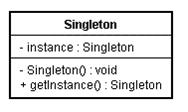
\includegraphics[scale=.9]{img/singleton-diagrama}
\caption{Diagrama de classe}
\end{figure}

No diagrama de classe apresentado anteriormente existe um atributo \textit{singleton} que é do tipo da própria classe. Nos métodos da classe podemos verificar a presença do construtor de classe, \textit{Singleton()}, que é privado. Ora, para que a classe seja instanciada é necessário utilizar o método estático \textit{getInstance()}, assim pode ser acedido por qualquer outra classe.

\begin{lstlisting}[caption=Solução de implementação]
public class MyClass {
  private static MyClass instance = null;

  private MyClass() {
  }

  public static MyClass getInstance() {
    if(instance==null) {
      instance = new MyClass();
    }
    return MyClass.instance;
  }
}
\end{lstlisting}

Com a implementação anterior assegurasse que ao tentar-se criar duas instâncias da mesma classe isso não é possível, pois o atributo \textit{instance} já não está a \textit{null}.

\paragraph{Vantagens}

É um \textit{Pattern} simples e é utilizado quando se pretende ter um acesso único e global para organizar os recursos.

\paragraph{Desvantagens}

A utilização exagerada deste \textit{pattern} pode provocar depedências muito fortes entre os objetos e dificultar alterações de configurações futuras.
